\begin{figure}[h!]
	\centering
	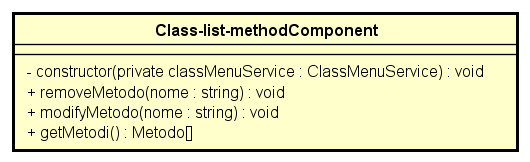
\includegraphics[scale=0.8]{res/sections/SpecificaFrontEnd/Components/Disegnetti/class-list-method.png}
	\caption{Diagramma della classe Class-list-method}
\end{figure}

\begin{itemize}
	\item \textbf{Descrizione:}\\
	
	\item \textbf{Utilizzo:}\\
	
	\item \textbf{Metodi:}
		\begin{itemize}
			\item \emph{-constructor(private classMenuService: ClassMenuService)}\\
    		Costruttore della classe\\
    		\textbf{Parametri:}
    		\begin{itemize}
    			\item \emph{classMenuService: ClassMenuService}\\
    			Crea un istanziazione di ClassMenuService
    		\end{itemize}
    		\item \emph{+removeMetodo(nome: string)}\\
    		Rimuove un metodo\\
    		\textbf{Parametri:}
    		\begin{itemize}
    			\item \emph{nome: string}\\
    			Nome del metodo da rimuovere
    		\end{itemize}
    		\item \emph{+modifyMetodo(nome: string)}\\
    		Modifica il corpo del metodo\\
    		\textbf{Parametri:}
    		\begin{itemize}
    			\item \emph{nome: string}\\
    			Nome del metodo
    		\end{itemize}
    		\item \emph{+getMetodi()}\\
    		Ritorna la lista dei metodi
		\end{itemize}
\end{itemize}